\documentclass[
  UTF8,
  xcolor={dvipsnames,rgb},
  hyperref={colorlinks, citecolor=orange, linkcolor=black},
  ]{beamer}

% \documentclass[
%   UTF8,
%   xcolor={dvipsnames,rgb},
%   hyperref={colorlinks, citecolor=orange, linkcolor=black},
%   ]{beamer}
\usepackage{xcolor}
\usepackage{appendixnumberbeamer}
\usepackage{bookmark}
\usepackage{ctex}
\usepackage{caption}
\usepackage{subfigure}
\usepackage{fontspec}
% \usepackage[english]{babel}
% \usepackage{csquotes}
\usepackage{amsmath}
\usepackage{amsthm}
\usepackage{unicode-math}
\usepackage{amssymb}
\usepackage{graphicx}
\usepackage{float}
\usepackage{color}
\usepackage[
    backend=biber,
    style=authoryear,
    sorting = nty,
    hyperref=true,
    doi=false
]{biblatex}

\setbeamerfont{footnote}{size=\tiny}

\usetheme[numbering=none]{Metropolis}

\usefonttheme{professionalfonts}
\setmainfont[Scale=1.0]{STIX Two Text}
\setsansfont[
    BoldFont={STIX Two Text SemiBold},
    ItalicFont={STIX Two Text Italic}
    ]{Arial}
\setmathfont{STIX Two Math}
\setCJKmainfont{KaiTi}[BoldFont=SimHei, ItalicFont=KaiTi]
\setCJKsansfont{KaiTi}[BoldFont=SimHei, ItalicFont=KaiTi]

\setbeamertemplate{caption}[numbered]
\setlength\bibitemsep{1.25\itemsep}

\setbeamertemplate{section in toc}[circle]
\setbeamertemplate{subsection in toc}[subsections numbered]
\setbeamertemplate{itemize item}[ball]
\setbeamertemplate{theorems}[ams style]
\setbeamertemplate{blocks}[rounded][shadow=true]
% \numberwithin{figure}{section}

\setbeamertemplate{footline}[frame number]

\theoremstyle{remark}
\newtheorem{assump}[theorem]{Identification Assumption}

\newenvironment{wideitemize}{\itemize\addtolength{\itemsep}{0.5em} }{\enditemize}

\title{Taming the Factor Zoo (JoF 2020) 论文讲解}
\date{\today}
% multiple authors
\author{王悦 \and 蒋金骋 \and 董轩逸}
\institute{金融机器学习第一组}

\begin{document}

\begin{frame}
    \maketitle
\end{frame}

\begin{frame}
    \tableofcontents
\end{frame}

\section{概述}

\begin{frame}
    \frametitle{核心问题}

    \begin{wideitemize}
        \item 研究目标:已知因子池 \(h_{t}\),如何检验新加入因子 \(g_{t}\) 是否在横截面上对资产价格具有解释力?
        \item 问题 \begin{enumerate}
            \item 检验哪个核心指标?
            \item \(h_{t}\) 中的因子已经很多,传统检验方法 (分组算收益率、GRS、Fama-MacBeth) 是否还能用?
            \item 计量上的问题:模型误设、遗漏变量,以及如何做推断
        \end{enumerate}
        \pause
        \item 本文的回应 \begin{enumerate}
            \item Cochrane(2009) 建议检验因子对于随机贴现因子载荷 (SDF loading) 的显著性
            \item 可能存在维数灾难的问题,需要对 \(h_{t}\) 进行变量筛选,使用 Double Selection LASSO (Belloni et al. 2014)
            \item 用CV进行参数精调,采用DS策略选因子,理论推导渐进分布,构建``plug-in''方差估计量
        \end{enumerate}
    \end{wideitemize}
\end{frame}

\begin{frame}
    \frametitle{本文的思路:Double Selection LASSO}

    % \begin{figure}[H]
    % \begin{center}
    % 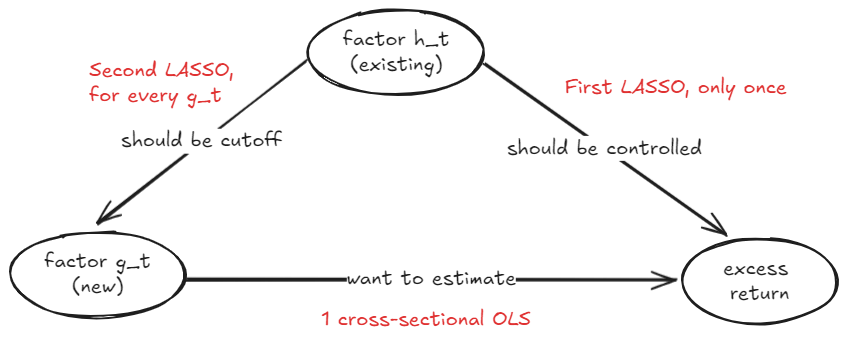
\includegraphics[width=0.8\textwidth]{../assets/idea.png}
    % \end{center}
    % \caption{研究思路}
    % \label{pic:1}
    % \end{figure}

    \begin{wideitemize}
        \item 第三步 (检验新因子):将 \textcolor{red}{\(N\) 个资产收益时序上的平均值}对\textcolor{blue}{控制因子 \(h_{t} \in \mathcal{I}_1 \cup \mathcal{I}_2\) 和新因子 \(g_{t}\) 和资产在时序上的协方差}在\textcolor{orange}{截面上进行OLS回归},得到 \(g_{t}\) 的SDF loading
        \item 第一步 (选控制因子):将 \textcolor{red}{\(N\) 个资产收益时序上的平均值}对\textcolor{blue}{控制因子 \(h_{t}\) 和资产在时序上的协方差}进行LASSO回归,选出控制因子池 \(\mathcal{I}_1\)
        \item 第二步 (防止遗漏控制因子):将\textcolor{red}{控制因子 \(h_{t}\) 和资产在时序上的协方差}对\textcolor{blue}{新因子 \(g_{t}\) 和资产在时序上的协方差}进行LASSO回归,选出控制因子池 \(\mathcal{I}_2\)
        \item 得到第三步的估计量后,构建样本方差,做推断,判断新因子的解释能力
    \end{wideitemize}

\end{frame}

\begin{frame}
    \frametitle{本文的思路:Double Selection LASSO}

    \begin{figure}[H]
    \begin{center}
    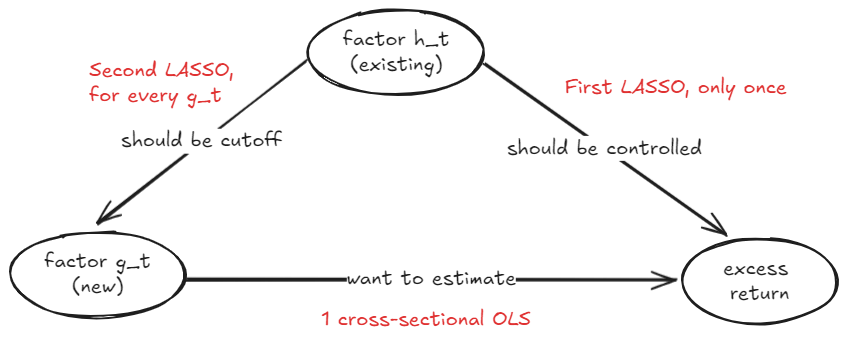
\includegraphics[width=0.9\textwidth]{../assets/idea.png}
    \end{center}
    \caption{研究思路}
    \label{pic:1}
    \end{figure}

\end{frame}

\section{理论模型}

\section{实证步骤}

\section{实证结果}

\end{document}